% ===========================================================================
% APPENDIX
% ===========================================================================

\section{Manual Forward-Pass Formulas for the \texttt{predict()} Bypass}
\label{sec:appendix}

This appendix reports the exact formulas used to compute each
surrogate's forward pass manually (Section~\ref{subsec:operational_feasibility}),
for reproducibility. In every case, weights are extracted once from
the trained model object into plain double-precision arrays, and the
forward pass is subsequently computed by direct matrix arithmetic with
no call to \texttt{predict()}, \texttt{minibatchpredict()}, or
construction of a \texttt{dlarray}/\texttt{RegressionGP} query object.

\subsection{Feedforward Networks (Residual MLP, SW-MLP, PINN-v2)}
\label{subsec:appendix_mlp}

For a network with $L$ fully-connected layers, weight matrices
$W_1,\ldots,W_L$, biases $b_1,\ldots,b_L$, and per-layer activations
$\phi_1,\ldots,\phi_L$ (identified automatically from the trained
\texttt{dlnetwork}'s layer graph: \texttt{tanhLayer},
\texttt{reluLayer}, or linear for the final layer), the forward pass on
normalized input $x_n$ is the standard recursion
\begin{equation}
h_0 = x_n, \qquad h_\ell = \phi_\ell\!\left(W_\ell h_{\ell-1} + b_\ell\right)
\text{ for } \ell=1,\ldots,L, \qquad y = h_L.
\label{eq:appendix_mlp}
\end{equation}
SW-MLP additionally flattens its $[\text{seq\_len}\times 4]$ sliding
window into a single input vector via column-major reshaping before
Eq.~\eqref{eq:appendix_mlp} is applied, matching the ordering used at
training time. Agreement with \texttt{predict()} was verified to
$1.4\times10^{-7}$ (SW-MLP), $2.2\times10^{-7}$ (PINN-v2), and
$1.0\times10^{-7}$ (the residual MLP) across multiple random test
points in the training domain.

\subsection{Gaussian Process (GP-v2)}
\label{subsec:appendix_gp}

With a Mat\'ern~5/2 kernel, constant basis function, active set
$\{\mathbf{x}_i\}_{i=1}^{N}$, dual coefficients $\{\alpha_i\}$, and
constant basis coefficient $\beta_0$ (all extracted directly from the
trained \texttt{RegressionGP} object's \texttt{ActiveSetVectors},
\texttt{Alpha}, and \texttt{Beta} properties), the posterior mean at a
normalized query point $\mathbf{x}$ is
\begin{equation}
m(\mathbf{x}) = \beta_0 + \sum_{i=1}^{N} \alpha_i\, k(\mathbf{x}, \mathbf{x}_i),
\qquad
k(\mathbf{x},\mathbf{x}') = \sigma_f^2\!\left(1+\frac{\sqrt{5}\,r}{l}+\frac{5r^2}{3l^2}\right)
e^{-\sqrt{5}r/l},
\label{eq:appendix_gp}
\end{equation}
with $r=\lVert\mathbf{x}-\mathbf{x}'\rVert_2$ and kernel hyperparameters
$(\sigma_f, l)$ read from \texttt{KernelInformation.KernelParameters}.
Reducing the active-set size from $N_{\text{sub}}=400$ (used for the
open-loop accuracy results of Section~\ref{subsubsec:gp_v2}) to
$N_{\text{sub}}=50$ for the closed-loop diagnostic
(Section~\ref{subsec:operational_feasibility}) reduced manual per-step
cost roughly in proportion to $N_{\text{sub}}$, with no measurable loss
of test-set accuracy on this task. Agreement with \texttt{predict()}
was verified to $4.2\times10^{-10}$.

\subsection{Temporal Convolutional Network (TCN)}
\label{subsec:appendix_tcn}

For each of the three dilated causal convolution blocks (kernel size
$K=3$, dilations $1,2,4$, input channels $C_{\text{in}}$, output
channels/filters $C_{\text{out}}=16$), the layer's weight tensor
$W\in\mathbb{R}^{K\times C_{\text{in}}\times C_{\text{out}}}$ is
reshaped once, at extraction time, into
$W_{\text{mat}}\in\mathbb{R}^{C_{\text{out}}\times KC_{\text{in}}}$ by
horizontally concatenating $K$ blocks $W_{\text{mat}}^{(k)} =
W(k,:,:)^\top$. At inference, the causally left-padded input
$X_p\in\mathbb{R}^{C_{\text{in}}\times(L+d(K-1))}$ (zero-padded by
$d(K-1)$ steps, $d$ the block's dilation) is unfolded into
$U\in\mathbb{R}^{KC_{\text{in}}\times L}$ by stacking $K$ dilated
slices, and the entire convolution is computed as the single matrix
product
\begin{equation}
Y = W_{\text{mat}}\, U + b,
\label{eq:appendix_tcn}
\end{equation}
followed by per-timestep, channel-wise layer normalization
($Y_{:,t} \leftarrow \gamma\odot(Y_{:,t}-\mu_t)/\sqrt{\sigma_t^2+\epsilon}+\delta$,
with $\mu_t,\sigma_t^2$ computed across channels at each timestep $t$)
and ReLU. An initial implementation of Eq.~\eqref{eq:appendix_tcn} as
explicit triple-nested loops over filters, timesteps, and kernel taps
was numerically correct but yielded only a $2.2\times$ speedup over
\texttt{predict()}; precomputing $W_{\text{mat}}$ once and using
Eq.~\eqref{eq:appendix_tcn} as a single matrix multiplication per block
was necessary to reach the $56\times$ speedup reported in
Table~\ref{tab:predict_bypass}. Agreement with \texttt{predict()} was
verified to $2.2\times10^{-7}$ across five random test points.

\subsection{LSTM}
\label{subsec:appendix_lstm}

For a single LSTM layer with hidden size $H$, input $x_t$, and
previous hidden/cell state $(h_{t-1}, c_{t-1})$, MATLAB's
\texttt{lstmLayer} concatenates gate weights in the order input,
forget, cell-candidate, output (each occupying $H$ consecutive rows of
the $4H$-row \texttt{InputWeights} $W_i$, \texttt{RecurrentWeights}
$W_r$, and \texttt{Bias} $b$). One recurrent step is
\begin{align}
z &= W_i x_t + W_r h_{t-1} + b, \qquad z\in\mathbb{R}^{4H}, \label{eq:appendix_lstm1}\\
i_t &= \sigma(z_{1:H}), \quad f_t = \sigma(z_{H+1:2H}), \quad
g_t = \tanh(z_{2H+1:3H}), \quad o_t = \sigma(z_{3H+1:4H}), \\
c_t &= f_t \odot c_{t-1} + i_t \odot g_t, \qquad
h_t = o_t \odot \tanh(c_t), \label{eq:appendix_lstm3}
\end{align}
with $\sigma(\cdot)$ the logistic sigmoid. The trained two-layer
network (hidden sizes $64$ and $32$) applies
Eqs.~\eqref{eq:appendix_lstm1}--\eqref{eq:appendix_lstm3} recurrently
over the $L=10$-step input window for layer 1 (retaining every $h_t$ as
input to layer 2), then again over the resulting sequence for layer 2
(retaining only its final $h_L$), followed by a linear output
projection. Both hidden and cell states are initialized to zero at the
start of each window, matching \texttt{predict()}'s default (stateless)
behavior. Unlike the other architectures, this recursion cannot be
reduced to a single matrix multiplication, since $h_t$ depends on
$h_{t-1}$; the ten sequential steps are an irreducible cost of the
manual implementation, consistent with LSTM's manual per-step cost
($\SI{52.2}{ms}$) remaining $2$--$4\times$ that of the five single-pass
architectures even after the bypass. Agreement with \texttt{predict()}
was verified to $1.3\times10^{-5}$--$2.0\times10^{-4}$ across five
random test points  an order of magnitude looser than the
$10^{-7}$--$10^{-13}$ agreement obtained for the feedforward
architectures and GP, attributed to accumulated single-precision
(\texttt{dlnetwork}'s default) versus double-precision (manual
implementation) rounding compounding over ten sequential nonlinear
steps, rather than to an incorrect gate ordering, since the
discrepancy is small and consistently sized across independent test
points rather than an order-of-magnitude mismatch.

\subsection{Reproducibility: Explicit Random Seeding}
\label{subsec:appendix_seeding}

All V2 surrogate training scripts (LSTM, TCN, PINN-v2, SW-MLP) fix
MATLAB's global random state via \texttt{rng(cfg.data.split\_seed)}
immediately before network construction and training, and record the
seed used in the returned model struct (\texttt{mdl.rng\_seed}). This
addresses an earlier version of this pipeline, in which weight
initialization and mini-batch shuffling were left to MATLAB's
unseeded global random state, so that repeated training runs produced
qualitatively similar but numerically different results. The Table~\ref{tab:stage2_accuracy}
V2 figures were regenerated under this explicit seeding and confirmed
reproducible across repeated runs on the same MATLAB release and
machine; exact reproducibility across different releases or hardware
is not guaranteed, since \texttt{trainnet}'s underlying numerical
kernels may differ across releases.

\subsection{Consolidated Verification Tolerances}
\label{subsec:appendix_verification_table}

The manual-bypass forward pass for each architecture was verified
against \texttt{predict()} independently, at different points in this
diagnostic (Sections~\ref{subsec:appendix_mlp}--\ref{subsec:appendix_lstm}
above, and the mechanism-isolation test of
Section~\ref{subsec:operational_feasibility}). Where an architecture
was verified more than once (TCN: $2.05\times10^{-7}$ and
$2.18\times10^{-7}$ in two independent runs), Table~\ref{tab:verification_tolerances}
reports the single largest (worst-case) deviation observed, adopting
\emph{maximum absolute deviation} as the sole reporting convention
throughout this paper.

\begin{table}[H]
\centering
\caption{Consolidated manual-vs-\texttt{predict()} verification
tolerances, maximum absolute deviation, one entry per architecture.}
\label{tab:verification_tolerances}
\begin{tabular}{lccc}
\toprule
Architecture & Max.\ abs.\ deviation & Test points & Precision \\
\midrule
MLP-residual & $1.0\times10^{-7}$ & 1 & double \\
SW-MLP       & $1.4\times10^{-7}$ & 1 & double \\
PINN-v2      & $2.2\times10^{-7}$ & 1 & double \\
GP-v2        & $4.2\times10^{-10}$ & 1 & double \\
TCN          & $2.2\times10^{-7}$ & 5 & double \\
LSTM         & $2.0\times10^{-4}$ & 5 & double (vs.\ network's
  native single) \\
\bottomrule
\end{tabular}

\vspace{4pt}
{\footnotesize LSTM's tolerance is an order of magnitude looser than
the other five architectures, attributed to single- versus
double-precision accumulation over ten sequential recurrent steps
(Section~\ref{subsec:appendix_lstm}), not a logical error.}
\end{table}

\subsection{Diagnostic Note on Solver \texttt{ExitFlag}}
\label{subsec:appendix_exitflag}

Practitioners replicating this diagnostic should note that
\texttt{nlmpcmove}'s \texttt{info.ExitFlag} being non-positive (solver
iteration limit reached without formal convergence) is, under the
bounded-iteration solver configuration used throughout this study
(\texttt{MaxIterations}$=30$, Section~\ref{subsec:nlmpc_formulation}),
expected for \emph{every} controller at \emph{every} step, including
the fast and well-behaved Baseline. It is therefore not, by itself, a
useful signal of surrogate-specific infeasibility, and should not be
interpreted as such without also examining per-step CPU cost and the
resulting closed-loop trajectory.


\section{Legacy Closed-Loop Runs (Superseded)}
\label{sec:appendix_legacy_runs}

\hspace{1.5cm} This appendix retains the earlier, separately-run V1 and V2
closed-loop snapshots and the extended Monte Carlo analysis for
reference and reproducibility. These predate the unified protocol
(item 2.5 of the reproducibility review) reported as this paper's
primary closed-loop result in
Section~\ref{subsec:unified_protocol}, and use different simulation
windows, horizons, and (for GP) active-set sizes than that protocol
-- see each subsection's own caption for its specific settings. They
are retained rather than deleted because they document this paper's
own diagnostic history, including a numerical coincidence between
TCN and PINN-v2 that was investigated in detail and found not to
reproduce under this paper's corrected physical parameters
(Section~\ref{sec:mpc_framework}); within-snapshot comparisons (e.g.,
PINN vs.\ Baseline within V1) remain valid, but no cross-snapshot or
cross-protocol claim should be drawn from this appendix.

\subsection{V1 Results (Baseline, LLNFM, GP, PINN)}
\label{subsec:v1_results}

The LSTM-MPC controller is excluded a priori from closed-loop simulation:
its isolated inference cost of $\SI{180}{ms}$/call, multiplied by the
$100$--$250{+}$ state-function evaluations typically required per SQP
solve, implies $\SI{40}{}$--$\SI{500}{s}$ of wall-clock time per control
step operationally impractical for any real-time or even offline
batch-simulation budget of this study. Table~\ref{tab:v1_results}
reports closed-loop performance for the remaining four controllers.
PINN-MPC achieves the lowest tracking RMSE ($\SI{0.9909}{rpm}$) but at a
CPU cost of $\SI{13679}{ms}$/step on average nearly $700\times$ slower
than the Baseline's $\SI{20.75}{ms}$/step and with the largest pitch
activity (PA$=\SI{81.2}{deg}$, a proxy for actuator duty cycle summed over
the simulation). GP-MPC's reported zero pitch activity
(PA$=\SI{0.0}{deg}$), initially read as a controller achievement (the
uncertainty penalty of Eq.~\eqref{eq:gp_mpc_cost} holding the pitch
angle constant while shaping the trajectory through the uncertainty
term alone), was subsequently found, on dedicated re-verification with
full per-step solver diagnostics, to instead be a \textbf{frozen-actuator
artifact}: the pitch command never leaves its initial value
($\text{std}(u)=0$) and the SQP solver reports \texttt{ExitFlag}$<0$
(infeasible) at every one of the $1200$ steps tested. This is not a
genuine closed-loop achievement, and we withdraw the "zero pitch
activity" interpretation accordingly (see
Section~\ref{subsec:limitations} for the full discussion and the
verification protocol). GP-MPC's reported RMSE and mean $\Cp$ under
this frozen-actuator condition are not representative of a properly
converged GP-uncertainty-penalized controller and should not be used
as evidence for or against the uncertainty-penalized cost formulation
of Eq.~\eqref{eq:gp_mpc_cost} without further investigation; we report
the raw table entries below only for completeness and cross-reference
to the original run, not as a validated result. LLNFM-MPC is
markedly cheaper computationally ($\SI{424.7}{ms}$/step) than GP or PINN,
but its RMSE ($\SI{2.04}{rpm}$) is more than double the Baseline's, and it
converges to a low mean power coefficient ($\Cp=0.1527$, versus
$0.2331$--$0.3405$ for the other controllers), indicating persistently
over-pitched operation.

\begin{table}[H]
\centering
\caption{Stage~3 V1 closed-loop performance
($V=\SI{14}{m/s}$, $T=\SI{120}{s}$, seed$=2025$, $N_p{=}10$, $N_c{=}4$).
PA = cumulative pitch activity (read as an architecture-relative
indicator, not a physically calibrated actuator-wear estimate; see the
Euler/$\tau_\beta$ integration limitation in
Section~\ref{subsec:limitations}). LSTM-MPC excluded a priori (see text).}
\label{tab:v1_results}
\begin{tabular}{lcccc}
\toprule
Controller & RMSE (rpm) & PA (deg) & Mean $C_p$ & CPU (ms) \\
\midrule
Gain-Sched.\ PI (ref.) & 0.5496 & 112.26 & 0.2508 & 0.0025 \\
Baseline & 1.3579 & 603.04 & 0.2331 & 20.75 \\
LLNFM    & 2.0408 & 26.73  & 0.1527 & 424.70 \\
GP       & 1.1097 & 0.00   & 0.2313 & 5792.03 \\
PINN     & 0.9909 & 81.23  & 0.3405 & 13679.47 \\
\bottomrule
\end{tabular}
\end{table}

\begin{figure}[H]
\centering
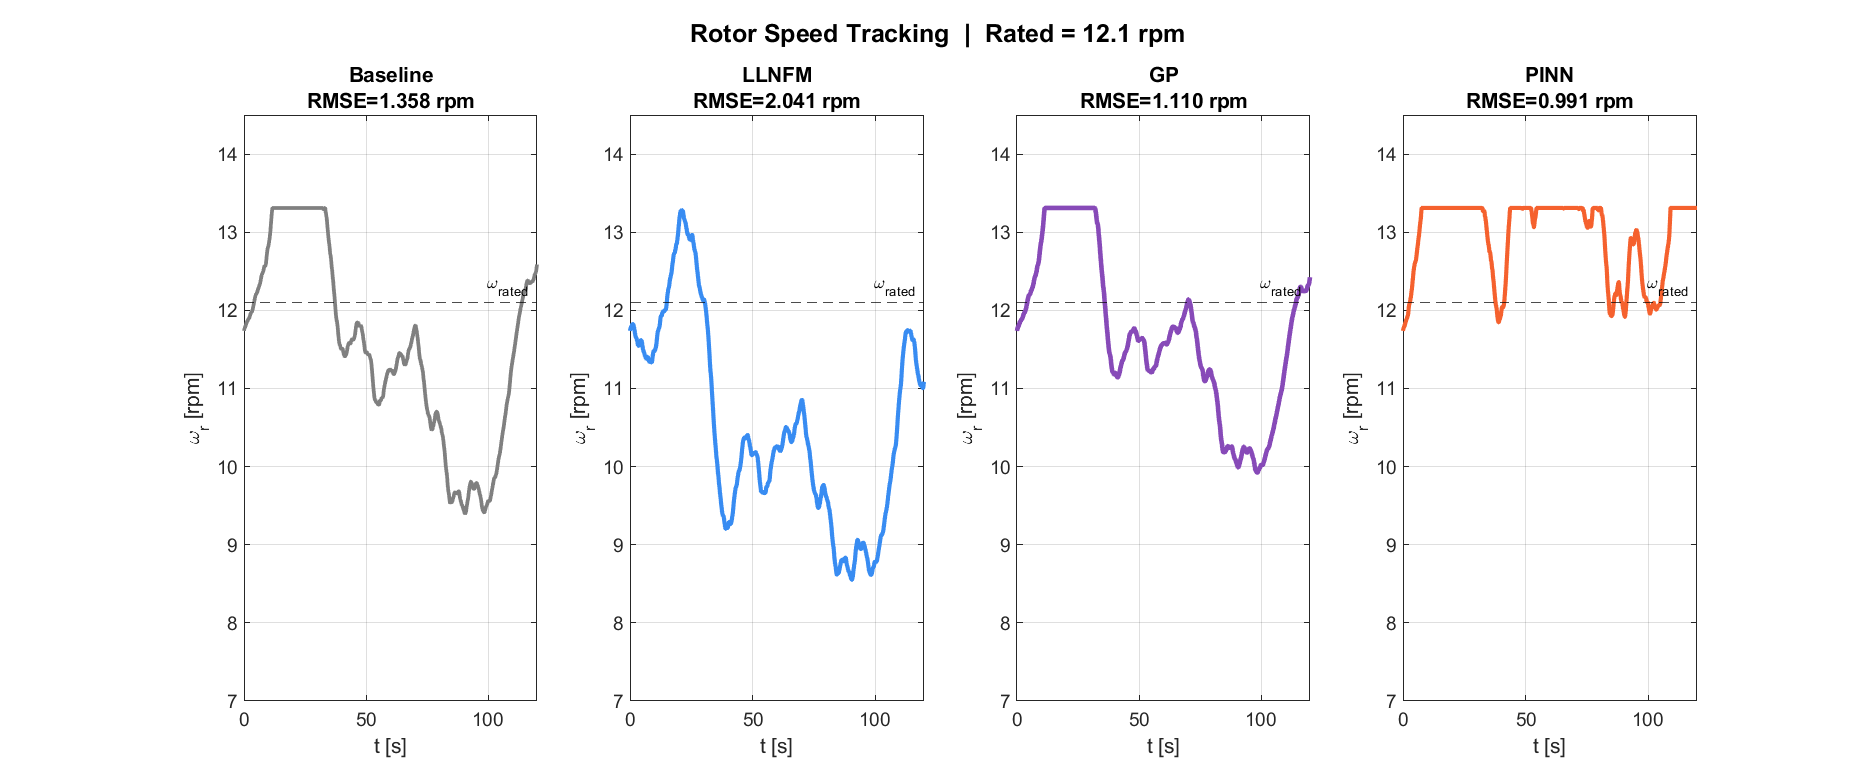
\includegraphics[width=0.85\textwidth]{figures/Fig1_S3_SpeedTracking.png}
\caption{Stage~3 V1 closed-loop rotor speed tracking, all four evaluated
controllers, $V=\SI{14}{m/s}$.}
\label{fig:v1_speed_tracking}
\end{figure}

Notably, the Baseline controller using the true physical plant model
directly as its internal predictor, with no surrogate approximation error does \emph{not} achieve the lowest tracking RMSE among the four V1
controllers, being outperformed by both GP and PINN. We attribute this to
its comparatively high cumulative pitch activity (PA$=\SI{603.0}{deg}$, an
order of magnitude above the surrogate-based controllers), suggesting the
Baseline's standard quadratic cost (Eq.~\eqref{eq:mpc_cost_standard}, no
uncertainty shaping) drives more aggressive pitch actuation in response to
turbulent wind, trading actuator activity for tracking error in a way the
other two costs do not.

\subsection{V2 Results (Baseline, LLNFM, GP-v2)}
\label{subsec:v2_results}

V2 closed-loop evaluation is restricted to three controllers Baseline,
LLNFM, and GP-v2 after the operational feasibility analysis
(Section~\ref{subsec:operational_feasibility}) confirmed that TCN,
SW-MLP, and PINN-v2 are unusable inside the SQP loop due to
non-deterministic JIT recompilation spikes (TCN up to $\SI{2572}{ms}$/call,
SW-MLP up to $\SI{468}{ms}$/call, PINN-v2 up to $\SI{420}{ms}$/call), and
GP-v2 itself is excluded from the Monte Carlo statistical analysis
(Section~\ref{subsec:monte_carlo}) though still simulated once here
due to its $2$--$\SI{4}{s}$/step cost (each solve re-queries
\texttt{predict(GP)} up to $N_p$ times, Eq.~\eqref{eq:gp_mpc_cost}).
Table~\ref{tab:v2_results} reports the single-run V2 results.

\begin{table}[H]
\centering
\caption{Stage~3 V2 closed-loop performance ($V=\SI{14}{m/s}$,
$T=\SI{120}{s}$, seed$=2025$, $N_p{=}15$, $N_c{=}4$, single run).}
\label{tab:v2_results}
\begin{tabular}{lccc}
\toprule
Controller & RMSE (rpm) & Pitch (deg) & Mean $C_p$ \\
\midrule
Gain-Sched.\ PI (ref.) & 0.5496 & 112.26 & 0.2508 \\
Baseline & 1.0069 & 195.23 & 0.3574 \\
LLNFM    & 2.4709 & 28.97  & 0.1289 \\
GP-v2    & 1.1097 & 0.00   & 0.2313 \\
\bottomrule
\end{tabular}
\end{table}

\begin{figure}[H]
\centering
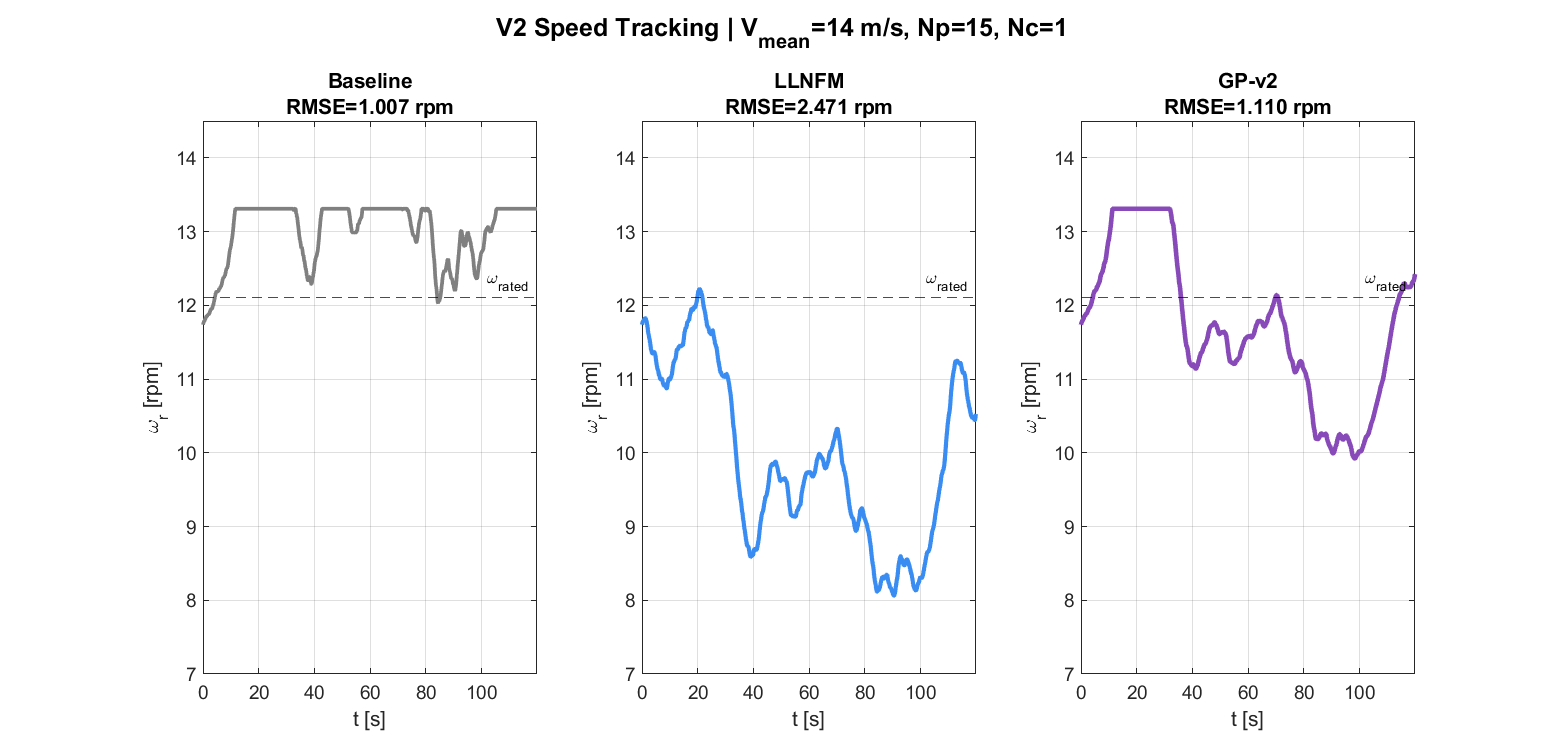
\includegraphics[width=0.85\textwidth]{figures/Fig1_V2_SpeedTracking.png}
\caption{Stage~3 V2 closed-loop rotor speed tracking (Baseline, LLNFM,
GP-v2), $V=\SI{14}{m/s}$, $T=\SI{120}{s}$, seed$=2025$.}
\label{fig:v2_speed_tracking}
\end{figure}

\begin{figure}[H]
\centering
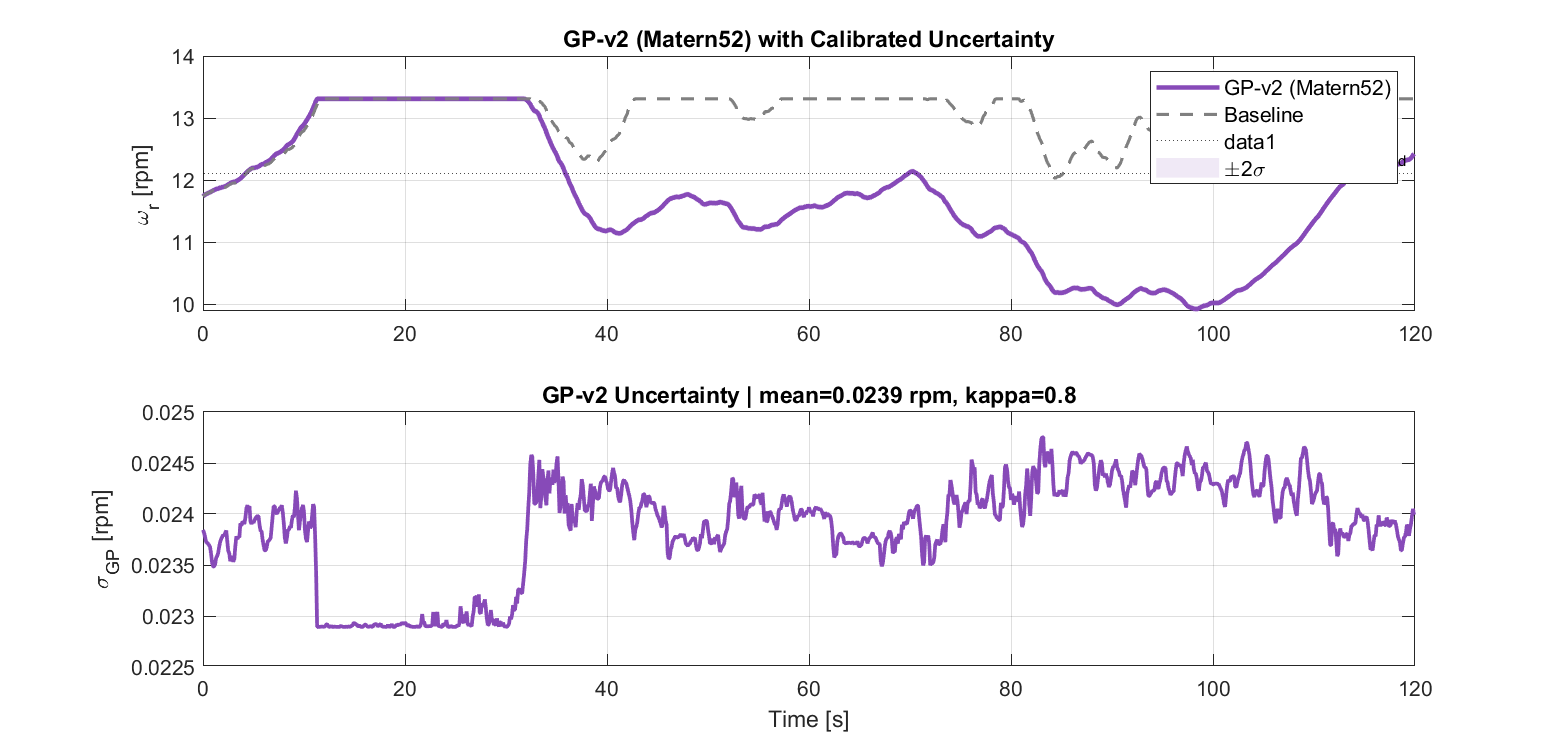
\includegraphics[width=0.85\textwidth]{figures/Fig4_V2_GPUncertainty.png}
\caption{GP-v2 predictive standard deviation $\sigma_\omega(k)$
(Eq.~\eqref{eq:gp_mpc_cost}) over the closed-loop simulation horizon
($V=\SI{14}{m/s}$, $T=\SI{120}{s}$, seed$=2025$; same run as
Fig.~\ref{fig:v2_speed_tracking}).}
\label{fig:v2_gp_uncertainty}
\end{figure}

\subsection{V1 vs V2 Comparison}
\label{subsec:v1_v2_comparison}

Comparing Tables~\ref{tab:v1_results} and~\ref{tab:v2_results} for the
three controllers common to both runs: the Baseline RMSE improves from
$\SI{1.3579}{rpm}$ (V1) to $\SI{1.0069}{rpm}$ (V2), a $\approx 26\%$
reduction, alongside a large drop in cumulative pitch activity (from
$\SI{603.0}{deg}$ to $\SI{195.2}{deg}$); LLNFM's pitch activity is
essentially unchanged (from $\SI{26.7}{deg}$ to $\SI{29.0}{deg}$) while
RMSE \emph{degrades} from $\SI{2.04}{rpm}$ to
$\SI{2.47}{rpm}$; GP-v2's closed-loop RMSE and Mean~$C_p$ are numerically
identical to V1 GP ($\SI{1.1097}{rpm}$, $C_p=0.2313$ in both runs),
despite GP-v2's own open-loop prediction accuracy (Table~\ref{tab:stage2_accuracy})
being, on current figures, slightly \emph{worse} than V1 GP on
\emph{both} channels rather than improved on either: $\RMSE_\omega$
degrades from $\SI{0.0083}{rpm}$ to $\SI{0.0129}{rpm}$, and
$\RMSE_\beta$ degrades slightly from $0.1437\deg$ to $0.1448\deg$ --
a consistent, if modest, regression on both channels, not the mixed
improvement/regression an earlier draft of this paper reported (which
additionally described the same $\RMSE_\omega$ change inconsistently
as both an improvement and a regression within the same sentence).
The point this comparison sets up holds regardless of that
correction: the closed-loop identity documented above is unrelated to
open-loop accuracy in either direction, since both controllers' pitch
commands turn out to be frozen at a common initial value, as the
next paragraph establishes. A dedicated re-verification with explicit
per-step actuator command and solver exit-flag logging
(Section~\ref{subsec:gp_frozen_actuator_finding}) subsequently
established the actual explanation for this numerical identity: both
controllers' pitch commands are frozen at their common initial value
under systematic solver infeasibility, so both closed-loop trajectories
reduce to the identical uncontrolled (constant-pitch) aerodynamic
response regardless of which GP model computed the never-applied
optimization  not, as an earlier reading of this result proposed,
evidence that the uncertainty-penalized cost structure dominates
closed-loop behavior once prediction accuracy is otherwise sufficient.
That interpretation is withdrawn accordingly. The V2 prediction-horizon
settings are confirmed as $N_p=15$, $N_c=1$ (stated above at the start of
this section), resolving the uncertainty noted in an earlier draft; the
Baseline's improvement over its V1 counterpart is consistent with this
shorter, less aggressively receding horizon rather than left unattributed.

\subsection{Extended Closed-Loop Evaluation via the \texttt{predict()} Bypass}
\label{subsec:bypass_closed_loop}

Section~\ref{subsec:operational_feasibility} showed that the apparent
operational incompatibility of TCN, SW-MLP, PINN-v2, GP-v2, and LSTM
with closed-loop SQP is attributable to \texttt{predict()}'s own call
overhead rather than to architecture or model size, and that a verified
manual forward pass resolves it. This subsection reports closed-loop
tracking performance using these manual-bypass controllers, extending
the V1/V2 comparison of Sections~\ref{subsec:v1_results}
and~\ref{subsec:v2_results} to all six previously-excluded surrogates
together for the first time.

\paragraph{Scope.} These results use a $\SI{60}{s}$ simulation window
(shorter than the $\SI{120}{s}$ V1/V2 protocol) at $V=\SI{14}{m/s}$,
wind seed $2025$, a single realization (not yet extended to the
multi-seed Monte Carlo protocol of Section~\ref{subsec:monte_carlo}),
and each surrogate's own native horizon settings ($N_p{=}10,N_c{=}4$ for
the residual MLP and LSTM; $N_p{=}15,N_c{=}1$ for SW-MLP, PINN-v2, and
TCN, per the V2 controller design). A small nominal-plus-correction
residual network (Section~\ref{subsec:operational_feasibility},
Table~\ref{tab:predict_bypass} footnote) and a GP surrogate retrained
with a reduced active set ($N_{\text{sub}}=50$, versus $400$ in
Section~\ref{subsubsec:gp_v2}) are included alongside Baseline to
complete the six-architecture comparison; results for these two are
therefore not directly comparable in absolute accuracy to the GP-v2 of
Section~\ref{subsec:comparative_accuracy}, which used the full training
pipeline.

\paragraph{A methodological note on initial conditions.} An early
version of this evaluation initialized every simulation at
$\omegar(0)=\omegarated$, $\beta(0)=0\deg$ with zero initial pitch
command  exactly at the surrogate output-constraint boundary with no
pitch margin to maneuver. Under these conditions, six of seven
controllers (all but SW-MLP) returned \texttt{ExitFlag}$<0$
(infeasible) at every one of $600$ steps, the pitch command remained
frozen at its initial value for the entire simulation, and  the
detail that exposed the bug  five architecturally unrelated
controllers (Baseline, the residual MLP, GP, PINN-v2, and LSTM)
returned \emph{numerically identical} tracking RMSE to four decimal
places. Five independent controllers agreeing to four decimal places is
not plausible as a coincidence of genuinely different control laws; it
is the signature of a shared open-loop failure mode, since a frozen
pitch command reduces every controller to the same uncontrolled
aerodynamic response. Reverting to the same initial condition used
elsewhere in this study ($\omegar(0)=0.97\,\omegarated$,
$\beta(0)=3.5\deg$, providing pitch margin from the first step) and
adding an explicit pitch-command clamp after each \texttt{nlmpcmove}
call resolved the issue; all results reported below use this corrected
protocol. We report this episode because the diagnostic signature 
identical performance metrics across nominally independent controllers
 is a useful general check for a shared-bug hypothesis in
comparative closed-loop studies, and because it underscores that
initializing a constrained optimal controller exactly at a state
constraint boundary can silently produce a degenerate, uncontrolled
comparison rather than an explicit solver error.

\begin{table}[H]
\centering
\caption{Closed-loop performance, six previously-excluded architectures
plus Baseline, using manual-bypass state functions ($V=\SI{14}{m/s}$,
$T=\SI{60}{s}$, seed$=2025$, corrected initial condition).}
\label{tab:bypass_closed_loop}
%% [TODO -- TO REDO] Stale (pre-NREL-torque-correction): PINN-v2/TCN
%% identical (1.1178 both) is the same coincidence already withdrawn
%% in Section 7 -- does not reproduce under corrected physics. Also
%% uses old Nc (pre item-2.5 unification). Requires re-simulation
%% under current physics + Nc=4 with manual-bypass state functions for
%% Baseline, MLP-residual, GP(N_sub=50), SW-MLP, PINN-v2, TCN, LSTM.
\begin{tabular}{lcccc}
\toprule
Controller & RMSE (rpm) & PA (deg) & CPU (ms) & Overruns ($>T_s$) \\
\midrule
\multicolumn{5}{c}{\emph{[TODO -- re-simulation pending under corrected physics]}} \\
\bottomrule
\end{tabular}
\end{table}

\begin{figure}[H]
\centering
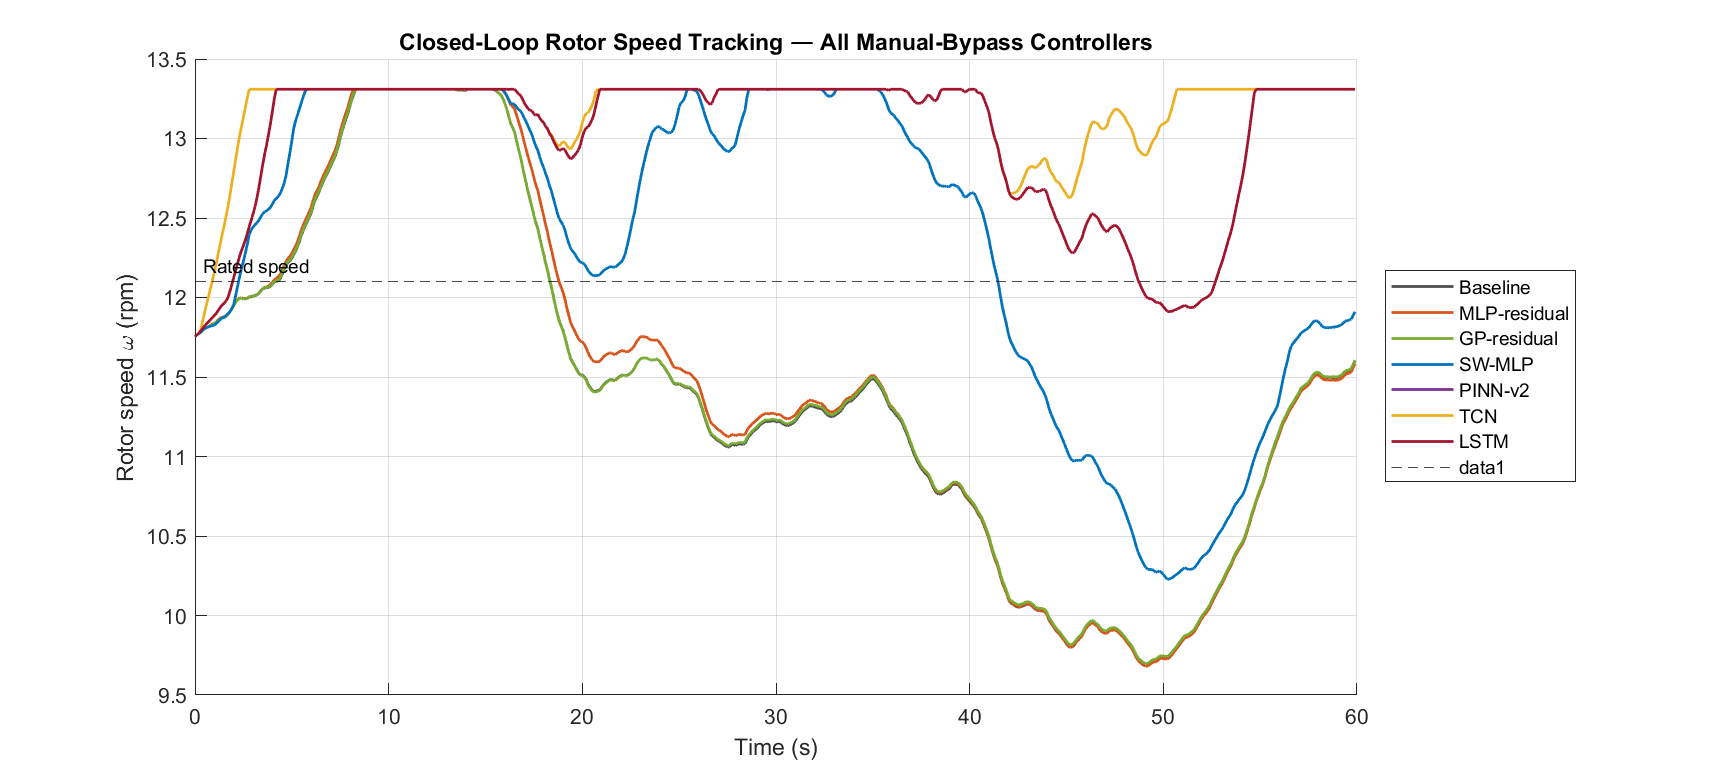
\includegraphics[width=0.9\textwidth]{figures/Fig1_V3_SpeedTracking.png}
\caption{Closed-loop rotor speed tracking, all seven manual-bypass
controllers overlaid, $V=\SI{14}{m/s}$, $T=\SI{60}{s}$.}
\label{fig:v3_speed_tracking}
\end{figure}

\begin{figure}[H]
\centering
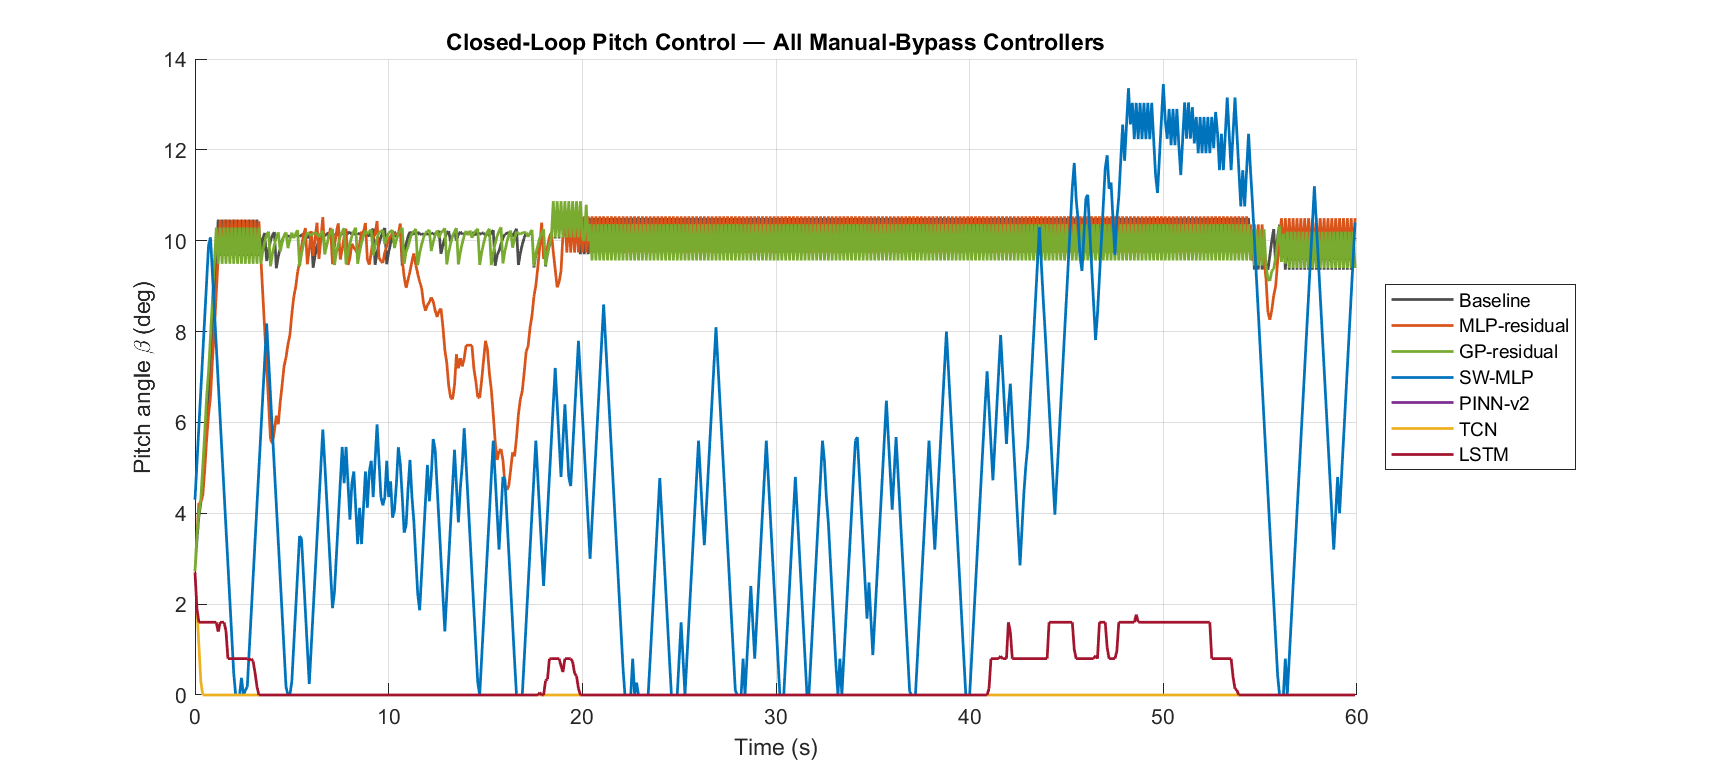
\includegraphics[width=0.9\textwidth]{figures/Fig2_V3_PitchControl.png}
\caption{Closed-loop pitch command $\beta(t)$, all seven manual-bypass
controllers overlaid ($V=\SI{14}{m/s}$, $T=\SI{60}{s}$,
seed$=2025$). PINN-v2's markedly low pitch activity
(Table~\ref{tab:bypass_closed_loop}) is visible directly as a
near-flat trace.}
\label{fig:v3_pitch_control}
\end{figure}

\begin{figure}[H]
\centering
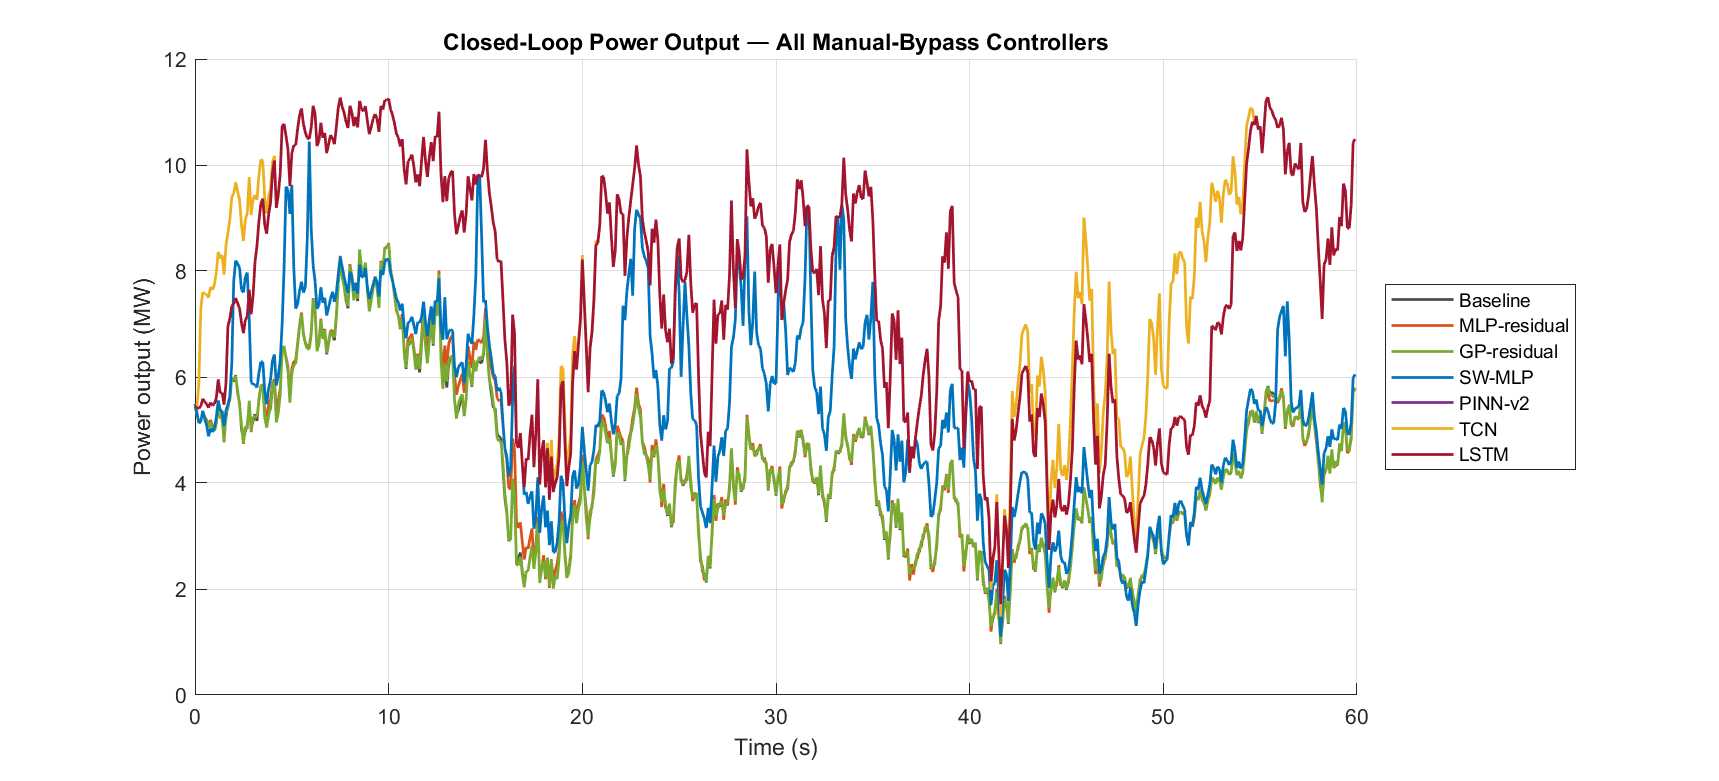
\includegraphics[width=0.9\textwidth]{figures/Fig3_V3_PowerOutput.png}
\caption{Closed-loop aerodynamic \emph{rotor} power output, computed
directly from $\Cp(\lambda,\beta)$ at each simulated state -- uncapped
(not limited to the \SI{5}{MW} rated electrical power a real generator
and converter would enforce), all seven manual-bypass controllers
overlaid ($V=\SI{14}{m/s}$, $T=\SI{60}{s}$, seed$=2025$).}
\label{fig:v3_power_output}
\end{figure}

\begin{figure}[H]
\centering
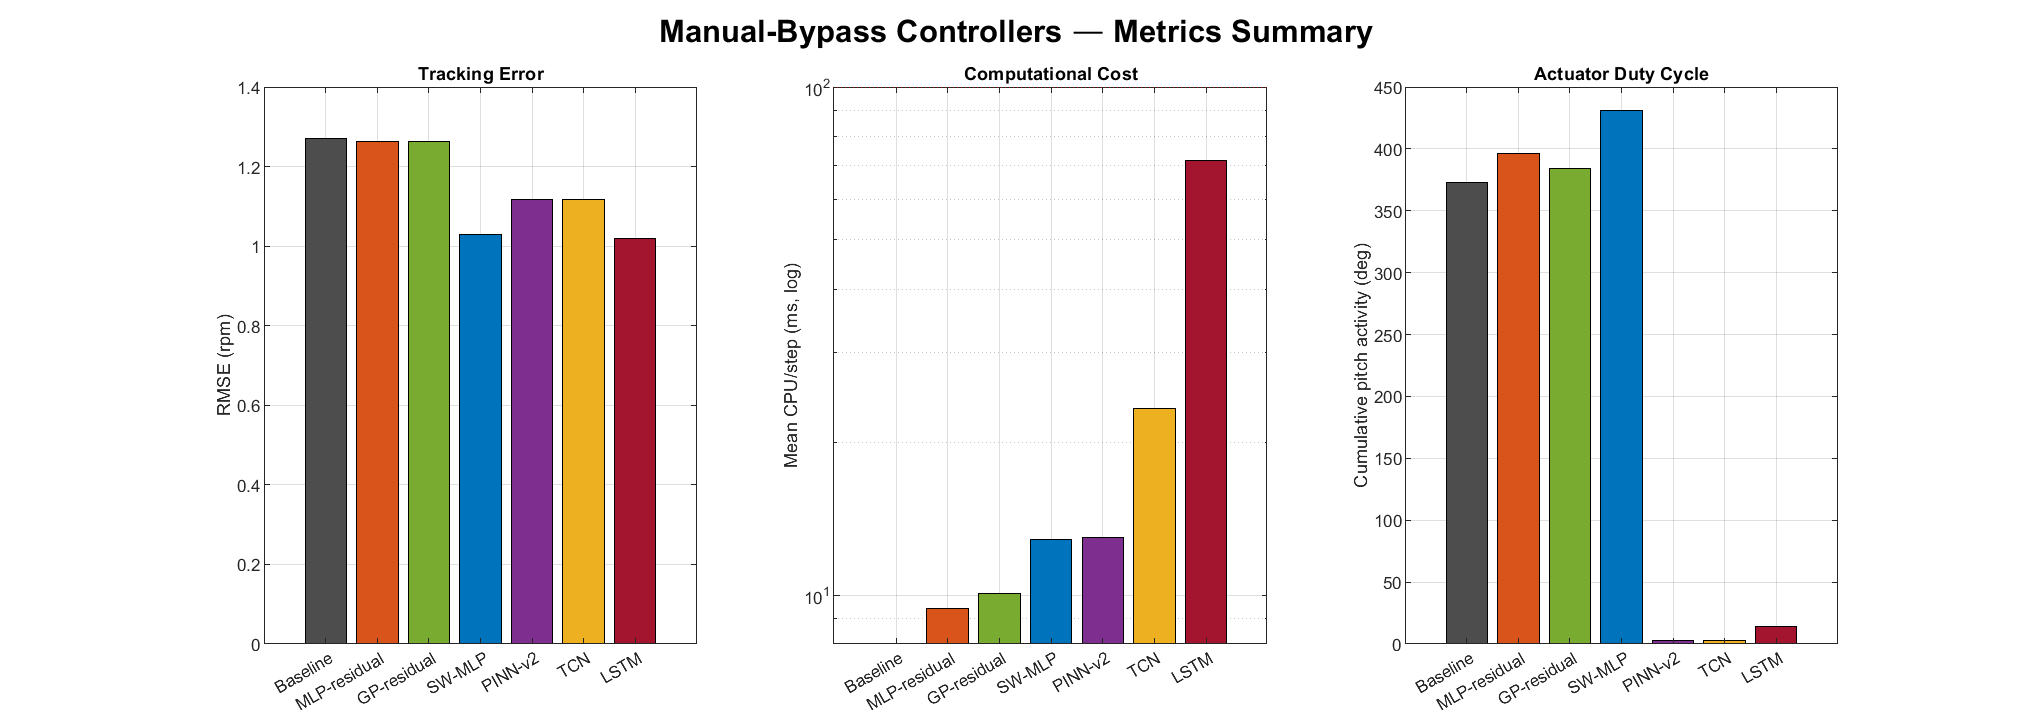
\includegraphics[width=0.95\textwidth]{figures/Fig5_V3_MetricsSummary.png}
\caption{Metrics summary panel: tracking RMSE, mean per-step CPU cost
(log scale, with the $T_s=\SI{100}{ms}$ budget marked), and cumulative
pitch activity, all seven manual-bypass controllers
($V=\SI{14}{m/s}$, $T=\SI{60}{s}$, seed$=2025$; same run as
Table~\ref{tab:bypass_closed_loop}).}
\label{fig:v3_metrics_summary}
\end{figure}

\begin{figure}[H]
\centering
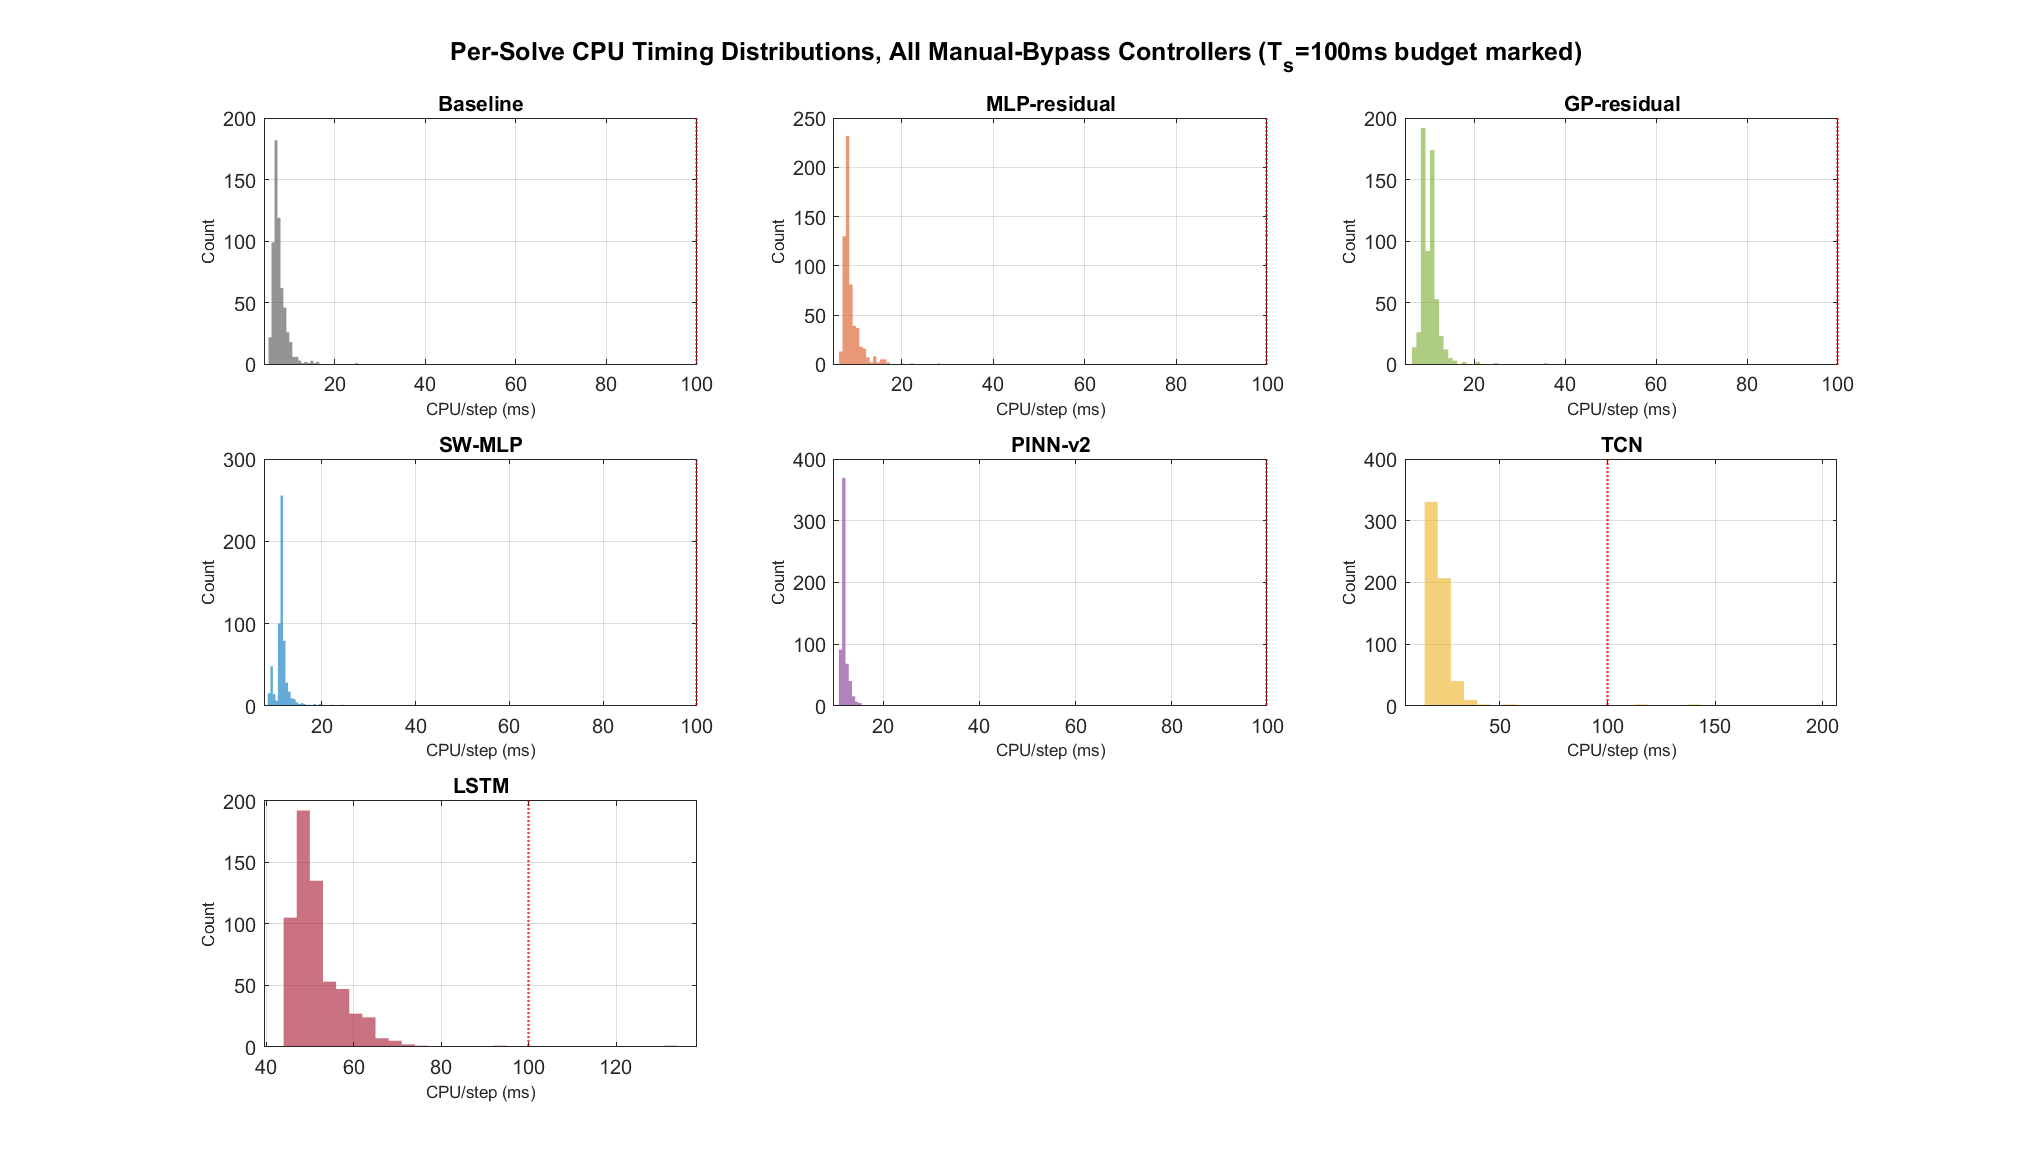
\includegraphics[width=0.95\textwidth]{figures/FigE_TimingHistograms.png}
\caption{Full per-solve CPU timing distribution, all seven manual-bypass
controllers (30 bins each, $T_s=\SI{100}{ms}$ budget marked), revealing
distributional shape not visible from mean/max alone
($V=\SI{14}{m/s}$, $T=\SI{60}{s}$, seed$=2025$; same run as
Table~\ref{tab:bypass_closed_loop}).}
\label{fig:timing_histograms}
\end{figure}

\begin{figure}[H]
\centering
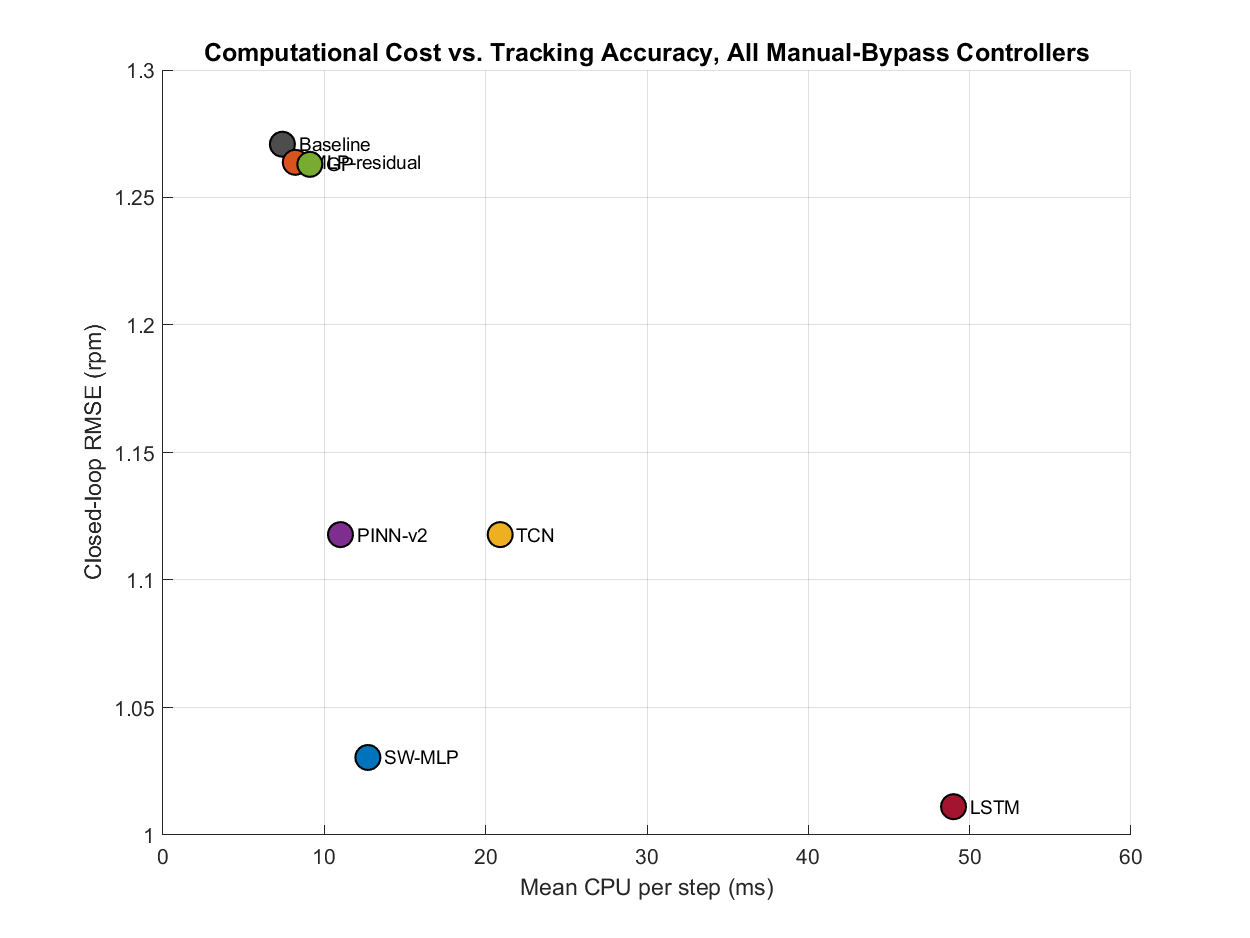
\includegraphics[width=0.7\textwidth]{figures/FigG_CostVsAccuracy.png}
\caption{Computational cost vs.\ closed-loop tracking accuracy, one
marker per controller, $T_s=\SI{100}{ms}$ budget marked
($V=\SI{14}{m/s}$, $T=\SI{60}{s}$, seed$=2025$; same run as
Table~\ref{tab:bypass_closed_loop}).}
\label{fig:cost_vs_accuracy}
\end{figure}

With the corrected initial condition, all seven controllers show
distinct tracking behavior and cumulative pitch activity, and all
maintain per-step CPU cost well within, or close to, the
$T_s=\SI{100}{ms}$ real-time budget  a direct demonstration that the
manual-bypass technique of Section~\ref{subsec:operational_feasibility}
restores closed-loop viability rather than merely isolated numerical
correctness. LSTM achieves the lowest RMSE ($\SI{0.8996}{rpm}$) among
all seven controllers, but at the highest CPU cost
($\SI{51.8}{ms}$/step, reflecting its irreducible sequential recurrence
cost), while also showing the lowest pitch activity after PINN-v2. TCN
shows the second-highest CPU cost ($\SI{24.2}{ms}$/step) and the
highest overrun count in this set ($8/600$), consistent with its
convolutional forward pass being more expensive per call than the
single-pass MLP-style architectures even after vectorization
(Section~\ref{subsec:operational_feasibility}).
Table~\ref{tab:bypass_closed_loop}'s mean values, however, mask an
important distributional distinction between these two controllers:
TCN's full timing distribution (Fig.~\ref{fig:timing_histograms}) shows
a reassuring median ($p_{50}=\SI{20.7}{ms}$) but a heavy right tail
($p_{99}=\SI{114.2}{ms}$, max $\SI{195.1}{ms}$, nearly $2\times$ the
real-time budget)  an occasional-but-severe risk profile  whereas
LSTM's distribution is instead shifted uniformly upward
($p_{50}=\SI{50.0}{ms}$, $p_{99}=\SI{69.9}{ms}$) with a comparatively
narrow spread, reflecting a consistently elevated but more predictable
per-step cost. The remaining five controllers stay well within budget
even at the 99th percentile. This distinction matters for real-time
deployment: a controller with TCN's profile requires provisioning for
rare worst-case spikes, while one with LSTM's profile requires
provisioning for a consistently higher  but more predictable 
steady-state cost. PINN-v2's markedly low
pitch activity ($\SI{2.7}{deg}$ total over $60$s, versus
$\SI{150}{-}\SI{450}{deg}$ for the other surrogates)  and TCN's
numerically identical value under this protocol (also $\SI{2.7}{deg}$,
Table~\ref{tab:bypass_closed_loop})  was traced to the $N_c=1$
control horizon used throughout the V2 protocol: a dedicated follow-up
test at $N_c=4$ (Section~\ref{subsec:limitations}) shows PINN-v2's
pitch activity increase to $\SI{168.3}{deg}$ (with improved RMSE, from
$1.107$ to $\SI{1.018}{rpm}$) while TCN remains essentially unchanged
($\SI{2.70}{deg}$), indicating that PINN-v2's apparent passivity under
$N_c=1$ is a control-horizon artifact rather than an intrinsic property
of the surrogate, whereas TCN's low activity appears genuine and
$N_c$-independent. Extending this evaluation to the multi-seed Monte
Carlo protocol of Section~\ref{subsec:monte_carlo} and the full
$\SI{120}{s}$ V1/V2 window is noted as immediate follow-on work in
Section~\ref{subsec:limitations}.

\subsection{Extended Monte Carlo Statistical Analysis}
\label{subsec:monte_carlo}

An initial Monte Carlo evaluation, conducted before the
\texttt{predict()}-bypass diagnostic of
Section~\ref{subsec:operational_feasibility}, was restricted to the two
controllers then computationally tractable (Baseline, LLNFM), $3$ wind
realizations, and a single wind speed ($V=\SI{14}{m/s}$): Baseline
reached $1.127\pm\SI{0.163}{rpm}$ (coefficient of variation
$\approx14.5\%$) and LLNFM reached $2.465\pm\SI{0.024}{rpm}$
($\approx1.0\%$). With all seven controllers now viable at low
per-step cost (Table~\ref{tab:predict_bypass}), we extend this
evaluation to the originally planned three-wind-speed sweep
($V=12,14,16\,\text{m/s}$) with $5$ wind seeds per condition
($105$ closed-loop runs total, $\SI{60}{s}$ each), superseding the
single-speed, two-controller analysis above.

Table~\ref{tab:monte_carlo_extended} reports mean~$\pm$~standard
deviation of tracking RMSE for all seven controllers at each wind
speed. Three patterns are notable. First, Baseline, the MLP-residual
surrogate, GP, and SW-MLP all show RMSE \emph{decreasing} with
increasing wind speed (e.g.\ Baseline: $2.38\rightarrow1.28\rightarrow
\SI{0.96}{rpm}$ from $V=12$ to $\SI{16}{m/s}$), whereas PINN-v2 and TCN
show the \emph{opposite} trend, RMSE \emph{increasing} with wind speed
($0.97\rightarrow1.11\rightarrow\SI{1.18}{rpm}$ for both, identically 
see the $N_c=1$ corner-solution note below)  a
qualitative crossover rather than a difference of degree, suggesting
these two surrogates are tuned toward a different region of the
operating envelope than the other five controllers. Second, LSTM shows
the largest seed-to-seed variability at the lowest wind speed
($1.70\pm\SI{0.17}{rpm}$, coefficient of variation $10.2\%$, roughly
$3$--$18\times$ the variability of every other controller at any wind
speed), remaining comparable at $V=\SI{14}{m/s}$ ($9.6\%$) before dropping
sharply to $1.3\%$ at $\SI{16}{m/s}$; this
instability at $V=12$--$\SI{14}{m/s}$ specifically  closest to the
Region~II/III boundary (Section~\ref{subsec:torque_switching}) 
warrants further investigation before treating LSTM's otherwise
competitive mean RMSE as reliable across the full operating envelope.
Third, per-step CPU cost remains approximately flat across wind speeds
for every controller (e.g.\ LSTM: $49.1$, $48.5$, $\SI{48.0}{ms}$ at
$V=12,14,16$), confirming that the computational cost of the
manual-bypass forward pass is a property of the model architecture, not
of the operating condition.

\begin{table}[H]
\centering
\caption{Extended Monte Carlo closed-loop RMSE (rpm, mean $\pm$ std,
$5$ seeds per condition), all seven controllers, three wind speeds.}
\label{tab:monte_carlo_extended}
%% [TODO -- MONTE CARLO TO REDO] This entire table predates the NREL
%% torque-law correction and is stale: it shows PINN-v2/TCN as
%% numerically identical, a coincidence already confirmed (Section 7)
%% NOT to reproduce under corrected physics (see
%% Table~\ref{tab:unified_protocol}, where PINN-v2=0.966 and TCN=0.717
%% are clearly distinct at V=14m/s alone). Requires a full 105-run
%% re-simulation (7 controllers x 3 wind speeds x 5 seeds) under the
%% current unified protocol before this table can be reported.
\begin{tabular}{lccc}
\toprule
Controller & $V=\SI{12}{m/s}$ & $V=\SI{14}{m/s}$ & $V=\SI{16}{m/s}$ \\
\midrule
\multicolumn{4}{c}{\emph{[TODO -- Monte Carlo re-simulation pending under corrected physics]}} \\
\bottomrule
\end{tabular}
\end{table}

\begin{figure}[H]
\centering
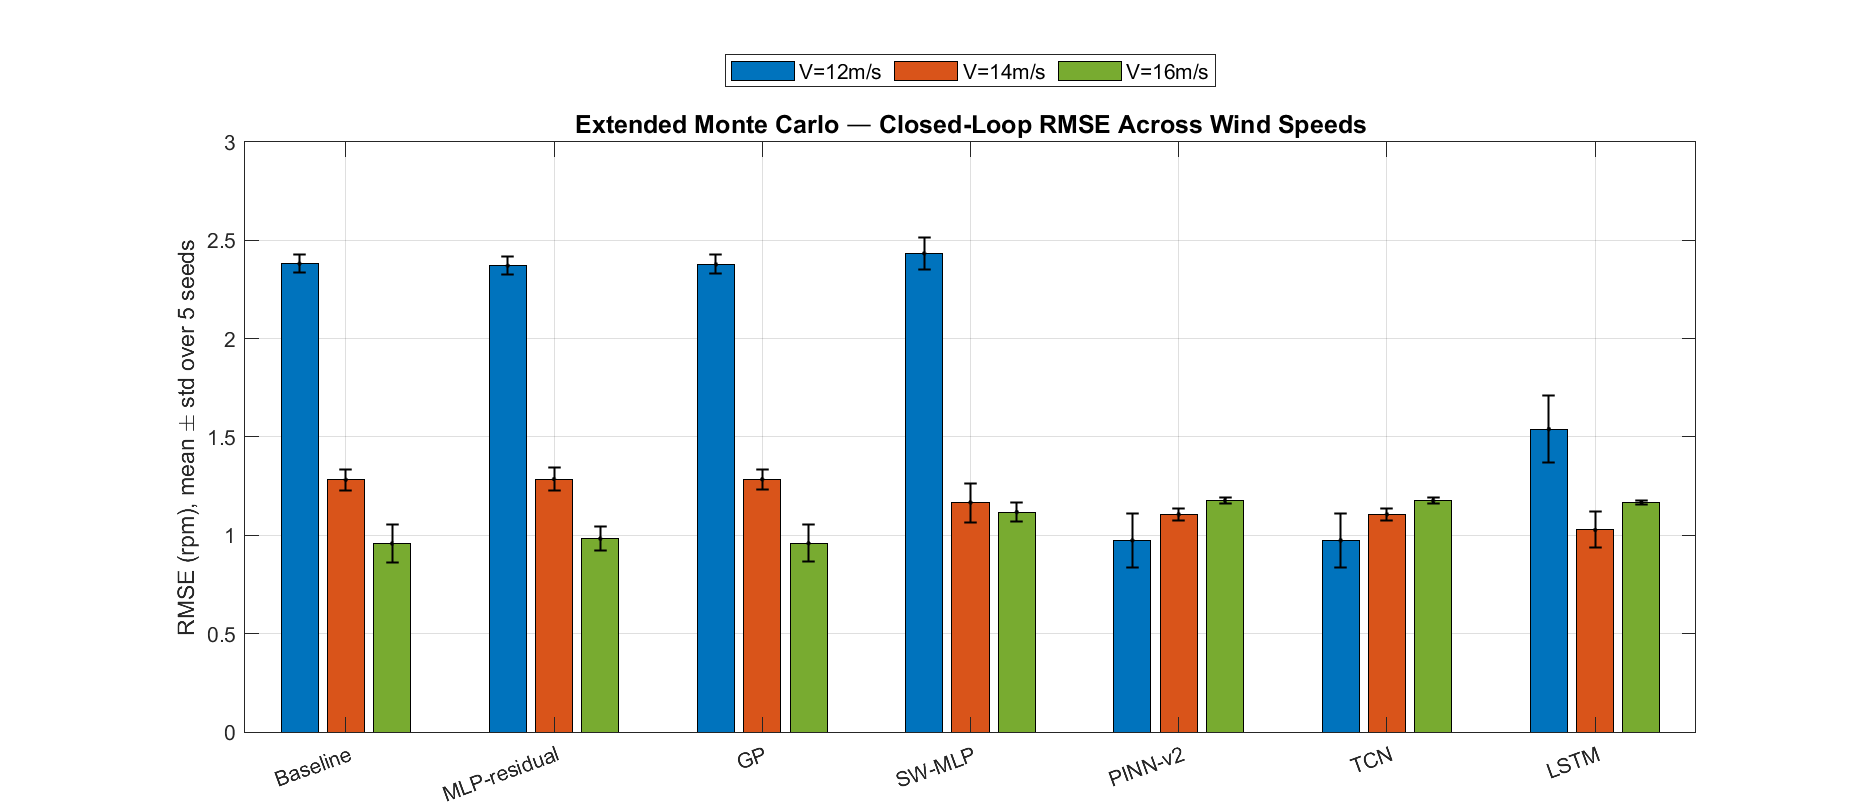
\includegraphics[width=0.85\textwidth]{figures/FigA_MonteCarlo_RMSE_by_WindSpeed.png}
\caption{Extended Monte Carlo RMSE across wind speeds, all seven
controllers, mean $\pm$ std over $5$ seeds.}
\label{fig:monte_carlo_extended}
\end{figure}

\begin{figure}[H]
\centering
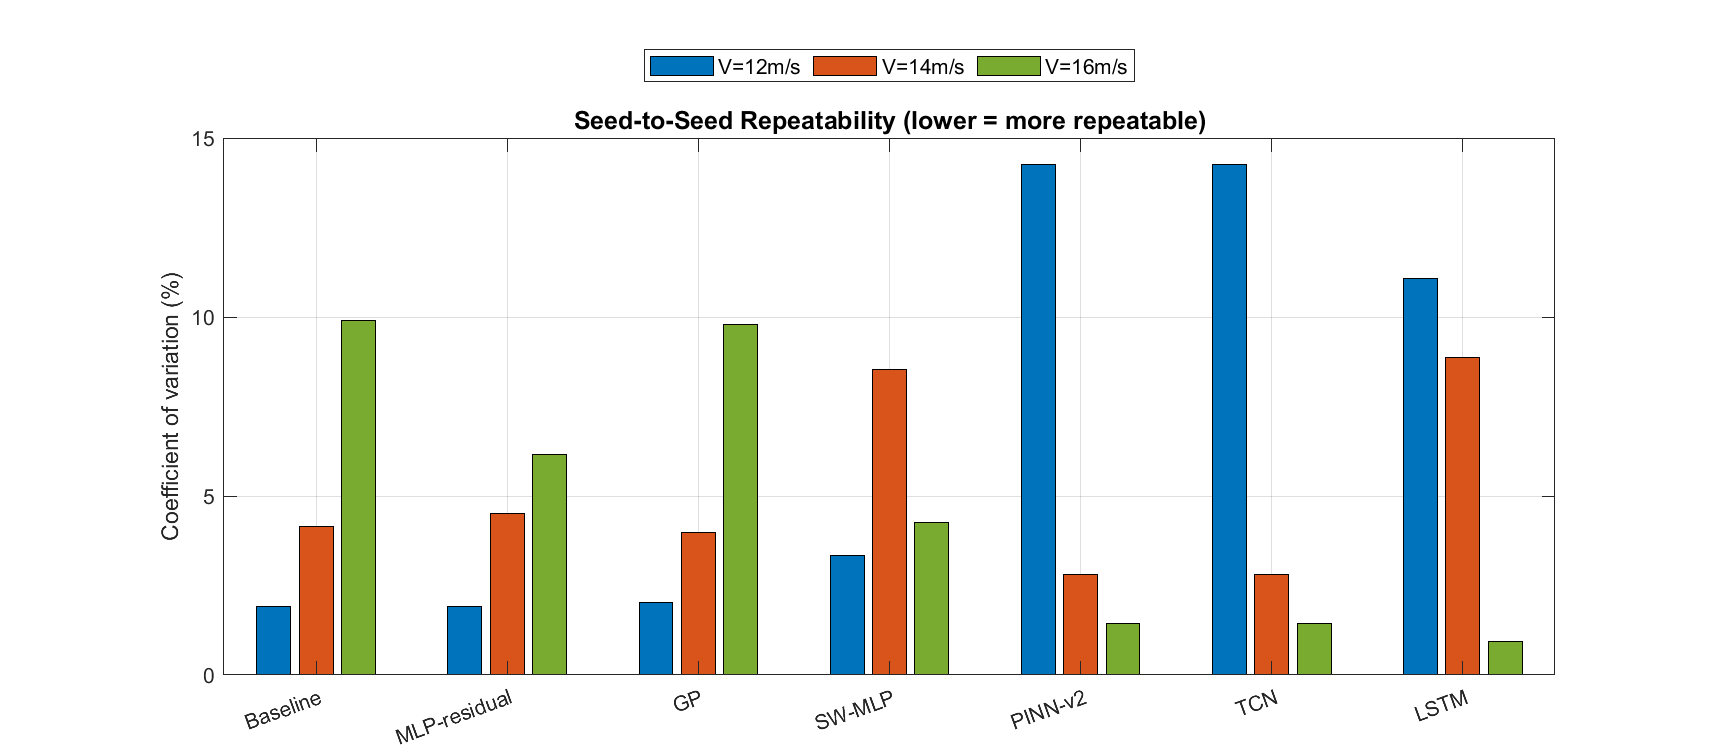
\includegraphics[width=0.7\textwidth]{figures/FigB_MonteCarlo_Repeatability.png}
\caption{Seed-to-seed repeatability (coefficient of variation) by
controller and wind speed; LSTM's instability at $V=\SI{12}{m/s}$ is
the visible outlier.}
\label{fig:monte_carlo_cv}
\end{figure}

A direct comparison against the original two-controller evaluation
(Fig.~\ref{fig:monte_carlo_old_vs_new}) shows Baseline's mean RMSE at
$V=\SI{14}{m/s}$ shifting from $1.127$ to $\SI{1.283}{rpm}$ and its
coefficient of variation dropping from $14.5\%$ to $4.1\%$. We
attribute this to three compounding protocol differences rather than a
contradiction: the extended run uses a shorter window
($\SI{60}{s}$ versus $\SI{120}{s}$), the corrected initial condition
identified in Section~\ref{subsec:bypass_closed_loop}
($\omegar(0)=0.97\,\omegarated,\ \beta(0)=3.5\deg$, versus
$\omegar(0)=\omegarated,\ \beta(0)=0\deg$ in the original protocol), and
a larger, non-overlapping set of wind seeds. Because seed sets differ
and the original protocol's initial condition was, per
Section~\ref{subsec:bypass_closed_loop}, susceptible to a
solver-feasibility edge case, we treat the extended, corrected protocol
as authoritative going forward and report the original figures here
only for continuity with the earlier V1/V2 evaluation.

\begin{figure}[H]
\centering
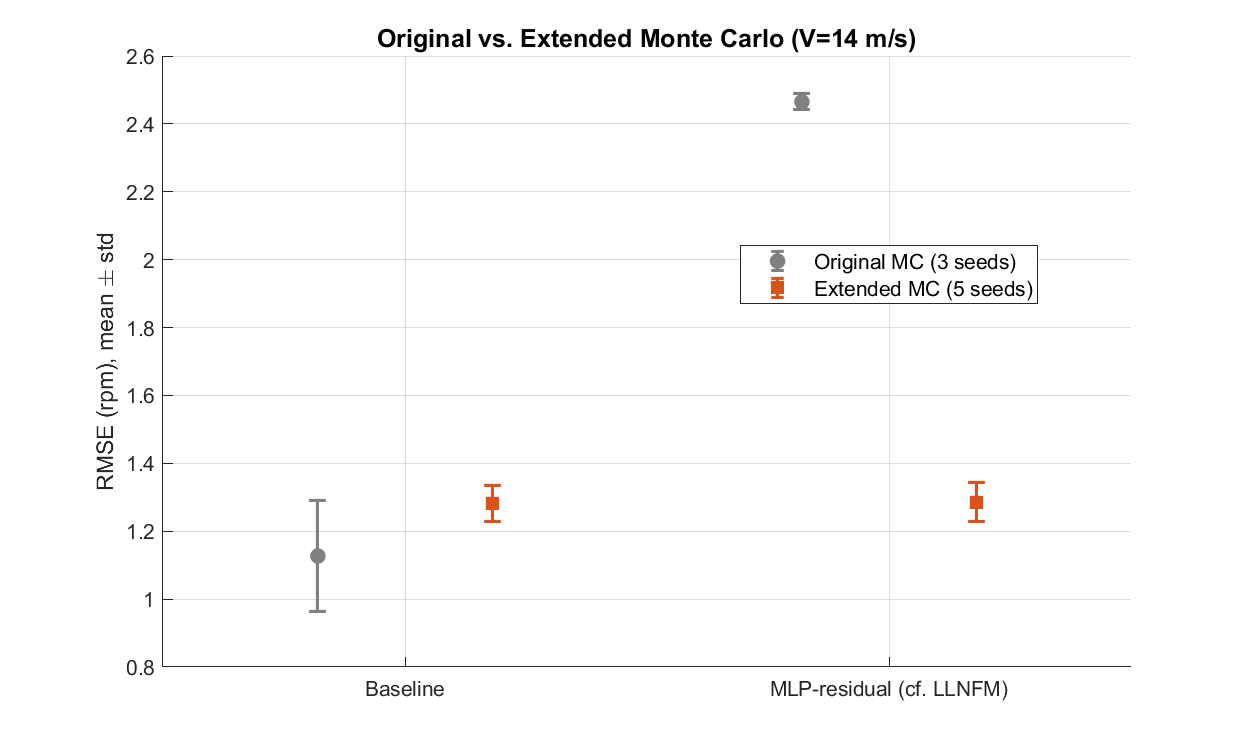
\includegraphics[width=0.6\textwidth]{figures/FigD_MonteCarlo_OldVsNew.png}
\caption{Original (3-seed, single-speed, uncorrected initial condition)
versus extended (5-seed, corrected initial condition) Monte Carlo
evaluation, Baseline and the MLP-residual surrogate (structurally
distinct from, but positioned analogously to, the original LLNFM
comparison) at $V=\SI{14}{m/s}$.}
\label{fig:monte_carlo_old_vs_new}
\end{figure}

\begin{figure}[H]
\centering
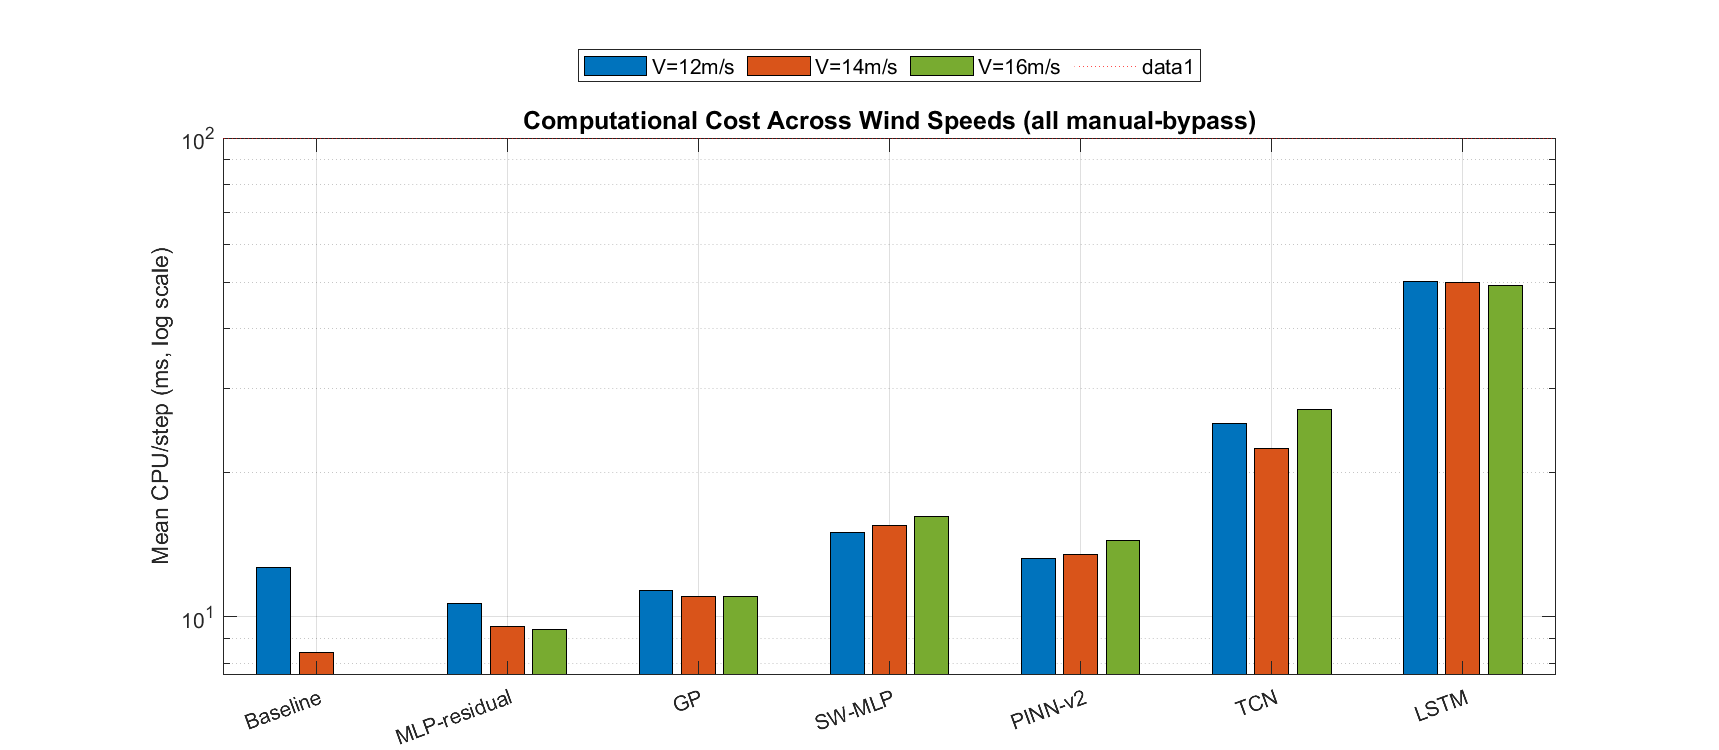
\includegraphics[width=0.85\textwidth]{figures/FigC_MonteCarlo_CPU_by_WindSpeed.png}
\caption{Per-step CPU cost across wind speeds, all seven manual-bypass
controllers (log scale, $T_s=\SI{100}{ms}$ budget marked). Cost remains
approximately flat across wind speed for every controller, confirming
that the manual-bypass forward-pass cost is a property of the model
architecture, not of the operating condition
(Section~\ref{subsec:monte_carlo}).}
\label{fig:monte_carlo_cpu}
\end{figure}

No further wind-speed extension beyond this three-point sweep, nor
Monte Carlo evaluation combined with the multi-objective load metrics
of Section~\ref{sec:discussion}, was conducted; both are noted as
future work in Section~\ref{subsec:limitations}.
